\documentclass[conference]{IEEEtran}
\IEEEoverridecommandlockouts

\usepackage{cite}
\usepackage{amsmath,amssymb,amsfonts}
\usepackage{algorithm}
\usepackage{algpseudocode}
\usepackage{booktabs} 
\usepackage{multirow}

\usepackage{graphicx}
\usepackage{textcomp}
\usepackage{xcolor}

\def\BibTeX{{\rm B\kern-.05em{\sc i\kern-.025em b}\kern-.08em
    T\kern-.1667em\lower.7ex\hbox{E}\kern-.125emX}}

\begin{document}

\title{A Validated Predictive-Prescriptive Framework for Automated Web Performance Optimization\\
}

\author{\IEEEauthorblockN{Shrimant Chavan}
\IEEEauthorblockA{\textit{Department of Computer Engineering} \\
\textit{COEP Technological University}\\
Pune, India \\
chavansa24.comp@coeptech.ac.in}
\and
\IEEEauthorblockN{Pratiksha Deshmukh}
\IEEEauthorblockA{\textit{Department of Computer Engineering} \\
\textit{COEP Technological University}\\
Pune, India \\
dpr.comp@coeptech.ac.in}
}

\maketitle

\begin{abstract}
Modern web applications demand proactive performance management, yet practitioners remain confined to reactive diagnostic tools. Lighthouse and similar auditors reveal \textit{that} a page is slow but offer no systematic path to resolution. This paper introduces a machine learning framework that unifies prediction, prescription, and explanation into a single automated pipeline. An XGBoost classifier trained on 885 webpages enriched with Core Web Vitals achieves 90.60\% accuracy and generalizes to 8,000 HTTP Archive URLs at 97.54\% accuracy. The classifier acts as a fitness function for a Differential Evolution optimizer that generates domain-compliant recommendations specifying both \textit{which} metrics to improve and \textit{by how much}. A consensus ranking reconciling SHAP, LIME, and Permutation Importance ensures transparent, stable explanations. Controlled real-world deployment validates the approach: implementing the prescribed changes reduced Largest Contentful Paint by 97.3\% and raised the Google PageSpeed score from 55 to 100---verified by an independent external audit. These results demonstrate a practical path from ML prediction to measurable production-level improvement.
\end{abstract}

\begin{IEEEkeywords}
Software Quality, Web Performance, Predictive Analytics, Explainable AI, Quality Assurance, Empirical Validation
\end{IEEEkeywords}

\section{Introduction}\label{sec1}

The performance of web applications is a decisive factor in the reliability and success of modern intelligent systems, directly dictating user satisfaction and operational efficiency. As web architectures evolve toward microservices and distributed cloud infrastructures, maintaining consistent low-latency performance has become a formidable engineering challenge \cite{kaushik2024, xin2023}. Modern applications rely heavily on dynamic content generation, where even minor degradation can severely impact business outcomes. Consequently, robust performance optimization has transitioned from a routine maintenance task to a critical requirement in intelligent computing environments \cite{dakic2025}.

A valid question arises: if runtime tools like Lighthouse already report performance scores, why invest in a predictive model? The answer lies in the qualitative difference between reactive measurement and proactive intelligence. First, a predictive model enables \textit{pre-deployment estimation}: during build time, before any page is live, the model forecasts the performance category, allowing issues to be flagged in CI/CD pipelines rather than discovered in production. Second, classification unlocks \textit{prescriptive search}: once a model acts as a differentiable objective, optimizers can explore the feature space to find minimal adjustments that shift a ``Slow'' prediction to ``Fast''. Third, prediction supports \textit{what-if analysis}: developers can simulate the impact of proposed changes without incurring the latency or quota limits of repeated Lighthouse calls.

Traditional optimization approaches remain predominantly manual and reactive, often depending on static heuristics that fail to capture the multidimensional nature of web behavior. To address these inefficiencies, recent research has pivoted toward data-driven modeling. Machine learning techniques have demonstrated significant potential in identifying performance patterns and predicting bottlenecks before they impact end-users \cite{ghattas2025, mathur2024}. However, a critical gap remains: most existing studies focus strictly on \textit{predicting} performance states, offering limited guidance on how developers should practically intervene to resolve identified issues. While predictive analytics provides an early warning system, engineers require prescriptive frameworks that recommend concrete, actionable optimization strategies \cite{notz2024}.

Furthermore, as machine learning models are deployed in performance-critical loops, the ``black-box'' nature of these algorithms raises concerns regarding transparency \cite{goyal2025}. Emerging surveys emphasize that for AI to be trusted in enterprise applications, it must provide interpretable reasoning via Explainable AI (XAI) techniques \cite{hassija2024, mersha2024}. Despite this, few studies have successfully integrated explainability into a unified pipeline that handles diagnosis, optimization, and justification simultaneously.

Motivated by these challenges, this research proposes an integrated framework that combines predictive modeling, prescriptive optimization, and explainable AI. Unlike purely theoretical studies, this work bridges the gap between AI strategy and engineering practice via a three-phase methodology: (1) an XGBoost-based classifier that categorizes performance using enriched Core Web Vitals; (2) a Differential Evolution optimization engine that prescribes domain-compliant feature adjustments; and (3) an XAI layer that validates these decisions using SHAP and LIME. Crucially, we validate the framework through a controlled real-world experiment, where AI-guided optimizations reduced Largest Contentful Paint (LCP) by 97.3\% and improved Google PageSpeed scores from 55 to 100. This empirical validation ensures that the proposed solution is practically viable for modern web engineering.

\section{Literature Review}

The optimization of web performance has evolved from static, rule-based heuristics to dynamic, data-driven methodologies. This section reviews existing literature across three pillars: predictive modeling, prescriptive analytics, and explainable artificial intelligence (XAI), highlighting the gaps that this research addresses.

\subsection{Predictive Performance Modeling}
Recent studies have demonstrated the efficacy of machine learning in forecasting web performance metrics. Ghattas et al. \cite{ghattas2025} utilized supervised learning algorithms to classify web page performance, achieving high accuracy by analyzing structural DOM elements. Similarly, Mathur et al. \cite{mathur2024} proposed a predictive analytics framework using regression models to estimate load times based on network conditions. Sehwag \cite{sehwag2024} extended this by applying Deep Learning and NLP to predictively prefetch resources, reducing perceived latency. However, these approaches are primarily diagnostic; they identify \textit{that} a page is slow but do not explicitly calculate \textit{how} to modify feature values to achieve a desired performance state.

\subsection{Prescriptive Analytics and Optimization}
To bridge the gap between prediction and action, prescriptive analytics has emerged as a vital area of research. Notz et al. \cite{notz2024} introduced explainable subgradient tree boosting for prescriptive tasks, demonstrating how ML models can guide decision-making under constraints. In the context of web systems, evolutionary algorithms have been explored for hyperparameter tuning. Surianarayanan et al. \cite{surianarayanan2023} utilized optimization algorithms for resource allocation in cloud environments. Despite these advancements, existing prescriptive frameworks often remain theoretical simulations. There is a notable scarcity of studies that validate AI-generated prescriptions through real-world deployment on live web servers, a gap this paper addresses through empirical validation.

\subsection{Explainable AI (XAI) in Engineering}
As AI systems become more complex, the need for transparency has grown. Surveys by Mersha et al. \cite{mersha2024} and Hassija et al. \cite{hassija2024} emphasize that ``black-box'' models hinder adoption in reliability-critical engineering domains. While techniques like SHAP and LIME have been successfully applied in healthcare and finance, their integration into web performance engineering remains limited. Current tools often provide optimization scores (e.g., Lighthouse) without explaining the distinct contribution of specific features to the overall prediction, leaving developers without granular insights.

\subsection{Comparative Analysis}
Prior to detailing the comparison, we note recent work on LLM-based approaches to web optimization \cite{burg2026}. Such methods excel at DOM-level code generation once specific issues are identified. Our framework is complementary: the predictive model identifies \textit{what} needs to change at a feature level, providing the quantified targets LLMs need for code generation.

Table \ref{tab1} summarizes the comparison between state-of-the-art approaches and the proposed framework. While prior works excel in individual aspects---prediction, optimization, or theory---our framework unifies these into a coherent pipeline validated by real-world experimentation.

\begin{table}[htbp]
\caption{Comparison with State-of-the-Art Approaches}
\begin{center}
\begin{tabular}{|c|c|c|c|}
\hline
\textbf{Ref.}&\multicolumn{3}{|c|}{\textbf{Functional Capabilities}} \\
\cline{2-4} 
\textbf{Author} & \textbf{\textit{Predictive}}& \textbf{\textit{Prescriptive}}& \textbf{\textit{Explainable}} \\
\hline
Ghattas \cite{ghattas2025}& Yes & No & No \\
\hline
Notz \cite{notz2024}& Yes & Yes (Theory) & Yes \\
\hline
Sehwag \cite{sehwag2024}& Yes & No & No \\
\hline
\textbf{Proposed}& \textbf{Yes} & \textbf{Yes (Validated)} & \textbf{Yes} \\
\hline
\multicolumn{4}{l}{$^{\mathrm{a}}$Proposed work includes real-world validation.}
\end{tabular}
\label{tab1}
\end{center}
\end{table}

\section{Problem Definition and Framework}

Web application performance is the result of intricate dependencies between DOM structure, network latency, resource composition, and browser rendering logic. Current diagnostic tools often function as isolated observatories rather than reasoning engines. This research formalizes an end-to-end framework merging predictive modeling, prescriptive analytics, and Explainable AI (XAI) to bridge this gap.

\subsection{Problem Formulation}
Let $W=\{w_{1},w_{2},...,w_{n}\}$ represent a corpus of web applications. For each application $w_{i}$, we define a feature vector $X_{i}=\{x_{i1},x_{i2},...,x_{id}\}$ comprising structural, network, and runtime attributes. We define three distinct but interrelated tasks:

\subsubsection{The Predictive Task}
Learn a supervised mapping function $f_{\theta}:X_{i}\rightarrow y_{i}$, where $y_{i}\in \{\text{Fast, Medium, Slow}\}$ represents the performance class. This model must generalize effectively across diverse web architectures to reliably flag under-performing pages \cite{ghattas2025}.

\subsubsection{The Prescriptive Task}
Identify feasible feature modifications that maximize the probability of an optimal performance state. For a given instance $w_{i}$, we seek an optimized vector $X_{i}^{*}$:
\begin{equation}
X_{i}^{*} = \arg \max_{X} P(y=\text{Fast} | f_{\theta}(X))
\end{equation}
subject to domain-specific constraints (e.g., maintaining visual integrity or limiting asset reduction). This formulation operationalizes the predictive model as an objective function within a meta-heuristic search space \cite{notz2024}.

\subsubsection{The Explainability Task}
Generate transparent interpretations for both the initial classification $f_{\theta}(X_{i})$ and the prescribed optimization $X_{i}^{*}$. We employ feature attribution methods to quantify the impact of specific metrics on the model's decisions, ensuring the system remains trustworthy \cite{salih2024}.

\subsection{Conceptual Framework}
The proposed architecture, illustrated in Fig. \ref{fig1}, consists of four cohesive layers:
\begin{itemize}
    \item \textbf{Data Layer:} Fuses static dataset features with dynamic runtime metrics (Core Web Vitals) to create a holistic view of application performance.
    \item \textbf{Predictive Layer:} Implements XGBoost to map feature vectors to performance classes. It acts as an ``oracle'' for the optimization engine.
    \item \textbf{Prescriptive Layer:} A Differential Evolution engine that queries the predictive model to find optimal feature adjustments, navigating the trade-off between maximizing performance probability and adhering to realistic constraints.
    \item \textbf{Explainability Layer:} Utilizes SHAP for global feature importance and LIME for local instance interpretation, ensuring stable transparency across the pipeline.
\end{itemize}

\section{System Architecture}

The proposed framework integrates data acquisition, predictive modeling, prescriptive analytics, and explainable AI into a unified pipeline (Fig. \ref{fig1}). The architecture is designed to not only detect performance bottlenecks but to actively prescribe constraint-aware solutions.

\begin{figure}[htbp]
\centerline{\includegraphics[width=\linewidth]{fig1.png}}
\caption{System architecture of the proposed predictive-prescriptive explainable framework.}
\label{fig1}
\end{figure}

\subsection{Data Layer (Input Augmentation)}
Standard datasets often rely on static file characteristics (e.g., total byte size) which correlate poorly with perceived user experience. To resolve this, we implement a data enrichment module. We combine static structural attributes (e.g., DOM depth, resource counts) with real-world runtime metrics retrieved via the Google PageSpeed Insights API. This process augments the feature space with Core Web Vitals, specifically Largest Contentful Paint (LCP), Total Blocking Time (TBT), and Cumulative Layout Shift (CLS), ensuring the model trains on indicators that truly reflect perceived performance \cite{mathur2024}.

\subsection{Phase 1: Predictive Modeling}
The predictive layer serves as the analytical core. Following preprocessing (log-transformation and robust scaling), the enriched data is fed into an XGBoost classifier. XGBoost was selected over Random Forests and SVMs due to its superior handling of tabular data and non-linear feature interactions \cite{xin2023}. In this framework, the model performs two functions:
\begin{itemize}
    \item \textbf{Classification:} Categorizing pages into performance classes (Fast, Medium, Slow).
    \item \textbf{Objective Evaluation:} Acting as a ``fitness function'' for the optimization engine, estimating the probability of improvement for potential configuration changes.
\end{itemize}

\subsection{Phase 2: Prescriptive Optimization}
While prediction identifies the problem, Phase 2 solves it. The engine employs Differential Evolution (DE), a stochastic optimization algorithm, to search the feature space. Mathematically, it treats the feature vector of a slow page as a candidate solution and iteratively mutates it to maximize the predicted probability of the ``Fast'' class ($P(\text{Fast})$). Crucially, this search is bound by Domain Constraints (e.g., limits on image compression or script deferral) to ensure recommendations are physically implementable \cite{surianarayanan2023}.

\subsection{Phase 3: Explainability Module}
To bridge the trust gap, we integrate an Explainable AI (XAI) layer:
\begin{itemize}
    \item \textbf{SHAP (Global):} Identifies system-wide performance drivers (e.g., which metrics generally dominate classification).
    \item \textbf{LIME (Local):} Provides instance-specific reasoning, clarifying exactly why a specific recommendation (e.g., ``Reduce JS payload by 200KB'') was generated for a specific URL \cite{salih2024}.
\end{itemize}

\subsection{Real-World Validation Loop}
Unlike prior works that rely on internal validation, this framework includes an external verification step. Recommendations are deployed to a live testbed and re-audited using the external Google PageSpeed API, establishing a ground-truth feedback loop.

\section{Experimental Setup}

This section details the data acquisition, feature engineering, and experimental protocols. The design prioritizes reproducibility, ensuring that predictive models are trained on high-quality data and prescriptive recommendations are verified in a controlled, real-world environment.

\subsection{Dataset Construction and Enrichment}
To ensure a representative sample of modern web architectures, we constructed a dataset merging static structural records with dynamic runtime metrics. The initial corpus was sourced from a public Kaggle repository, providing baseline attributes such as DOM complexity and resource counts.
However, static features alone fail to capture user-perceived latency \cite{kaushik2024}. We augmented this data using the Google PageSpeed Insights API, increasing the dataset to 885 unique webpages. This enrichment introduced 20 engineered features, specifically focusing on Core Web Vitals: Largest Contentful Paint (LCP), Total Blocking Time (TBT), and Cumulative Layout Shift (CLS).

\subsection{Feature Engineering}
Raw telemetry data often contains noise and scaling disparities. We applied robust preprocessing:
\begin{itemize}
    \item \textbf{Derived Indicators:} Calculated ratio-based metrics (e.g., Bytes-per-Request) to capture resource efficiency.
    \item \textbf{Log-Transformation:} applied to skewed distributions like page load times to normalize variance.
    \item \textbf{Robust Scaling:} All numerical features were scaled to the Interquartile Range (IQR) to mitigate the influence of outliers \cite{xin2023}.
\end{itemize}

\subsection{Model Training Protocol}
We evaluated three supervised algorithms: Support Vector Machines (SVM), Random Forests (RF), and XGBoost. The dataset was partitioned into a 70:30 stratified split (619 training, 266 test samples) to preserve class distribution across Fast, Medium, and Slow categories. Hyperparameters were optimized using grid search cross-validation, with $F1$-score as the primary metric.

\subsection{Real-World Validation Setup}
A key innovation of this work is the external validation of AI prescriptions. We designed a controlled experiment:
\begin{enumerate}
    \item \textbf{Baseline (``Bad'') Page:} A test site engineered with performance anti-patterns (e.g., 6MB uncompressed images, blocking scripts, 500+ redundant DOM elements).
    \item \textbf{Optimized (``Good'') Page:} The metrics from the Baseline were fed into our Prescriptive Engine. The resulting recommendations were manually implemented to create an optimized variant.
    \item \textbf{Independent Audit:} Both deployments were audited using the external Google PageSpeed API to quantify the exact reduction in latency.
\end{enumerate}

\section{Results and Analysis}

This section evaluates the framework's predictive accuracy, optimization efficacy, and decision interpretability.

\subsection{Predictive Performance}
Among the evaluated models, XGBoost demonstrated superior performance, achieving a testing accuracy of 90.60\% and an F1-score of 0.9055. Detailed metrics (Precision: 0.9072, Recall: 0.9060) indicate a balanced ability to minimize false positives. The confusion matrix revealed particular robustness in identifying the ``Slow'' class, attributed to the model's effective utilization of non-linear interactions between TBT and LCP. To validate generalizability, the model was applied to 8,000 HTTP Archive URLs, achieving 97.54\% cross-dataset accuracy, demonstrating robust transfer learning capability.

\subsection{Prescriptive Optimization Outcomes}
The prescriptive engine (Phase 2) was tested on under-performing pages. The Differential Evolution optimizer successfully identified feature adjustments that increased the predicted probability of the ``Fast'' class ($P_{fast}$) from $<1\%$ to $>99.6\%$.
Critically, the optimizer prioritized domain-compliant reductions rather than theoretical impossibilities:
\begin{itemize}
    \item \textbf{Response Time:} Average reduction of 72.1\%.
    \item \textbf{Time to Interactive (TTI):} Average reduction of 62.7\%.
    \item \textbf{LCP:} Average reduction of 61.0\%.
\end{itemize}

\subsection{Feature-to-Action Mapping}
To bridge the gap between ML outputs and developer workflows, we provide an explicit mapping from metrics to engineering interventions. Table \ref{tabaction} shows the key translations. During the real-world validation, the prescriptive recommendation ``Reduce Page Size by 99.9\%'' was implemented via: (i) converting a 6~MB BMP to a 5~KB WebP image, and (ii) removing render-blocking scripts. This demonstrates how abstract feature targets translate to concrete code-level changes.

\begin{table}[htbp]
\caption{Feature-to-Action Mapping}
\begin{center}
\resizebox{\linewidth}{!}{%
\begin{tabular}{|c|p{5.5cm}|}
\hline
\textbf{Metric} & \textbf{Developer Action} \\
\hline
LCP $\downarrow$ & Compress/convert hero images (WebP/AVIF), preload critical assets \\
\hline
TTI $\downarrow$ & Defer non-critical JS, code-split bundles \\
\hline
TBT $\downarrow$ & Break long tasks ($<$50ms), use web workers \\
\hline
Page Size $\downarrow$ & Minification, gzip/brotli, image optimization \\
\hline
\end{tabular}%
}
\label{tabaction}
\end{center}
\end{table}

\subsection{Explainability Analysis}
To validate trust, we employed a fidelity-weighted consensus ranking that reconciles three XAI techniques---SHAP, LIME, and Permutation Importance---into a single stable ranking. SHAP values computed via TreeExplainer identified Response Time, FCP, performance\_score, LCP, and Total\_Time as the five strongest global drivers. Figure~\ref{fig:shap} presents the global importance bar chart showing how Core Web Vitals dominate the model's decisions.

\begin{figure}[htbp]
\centerline{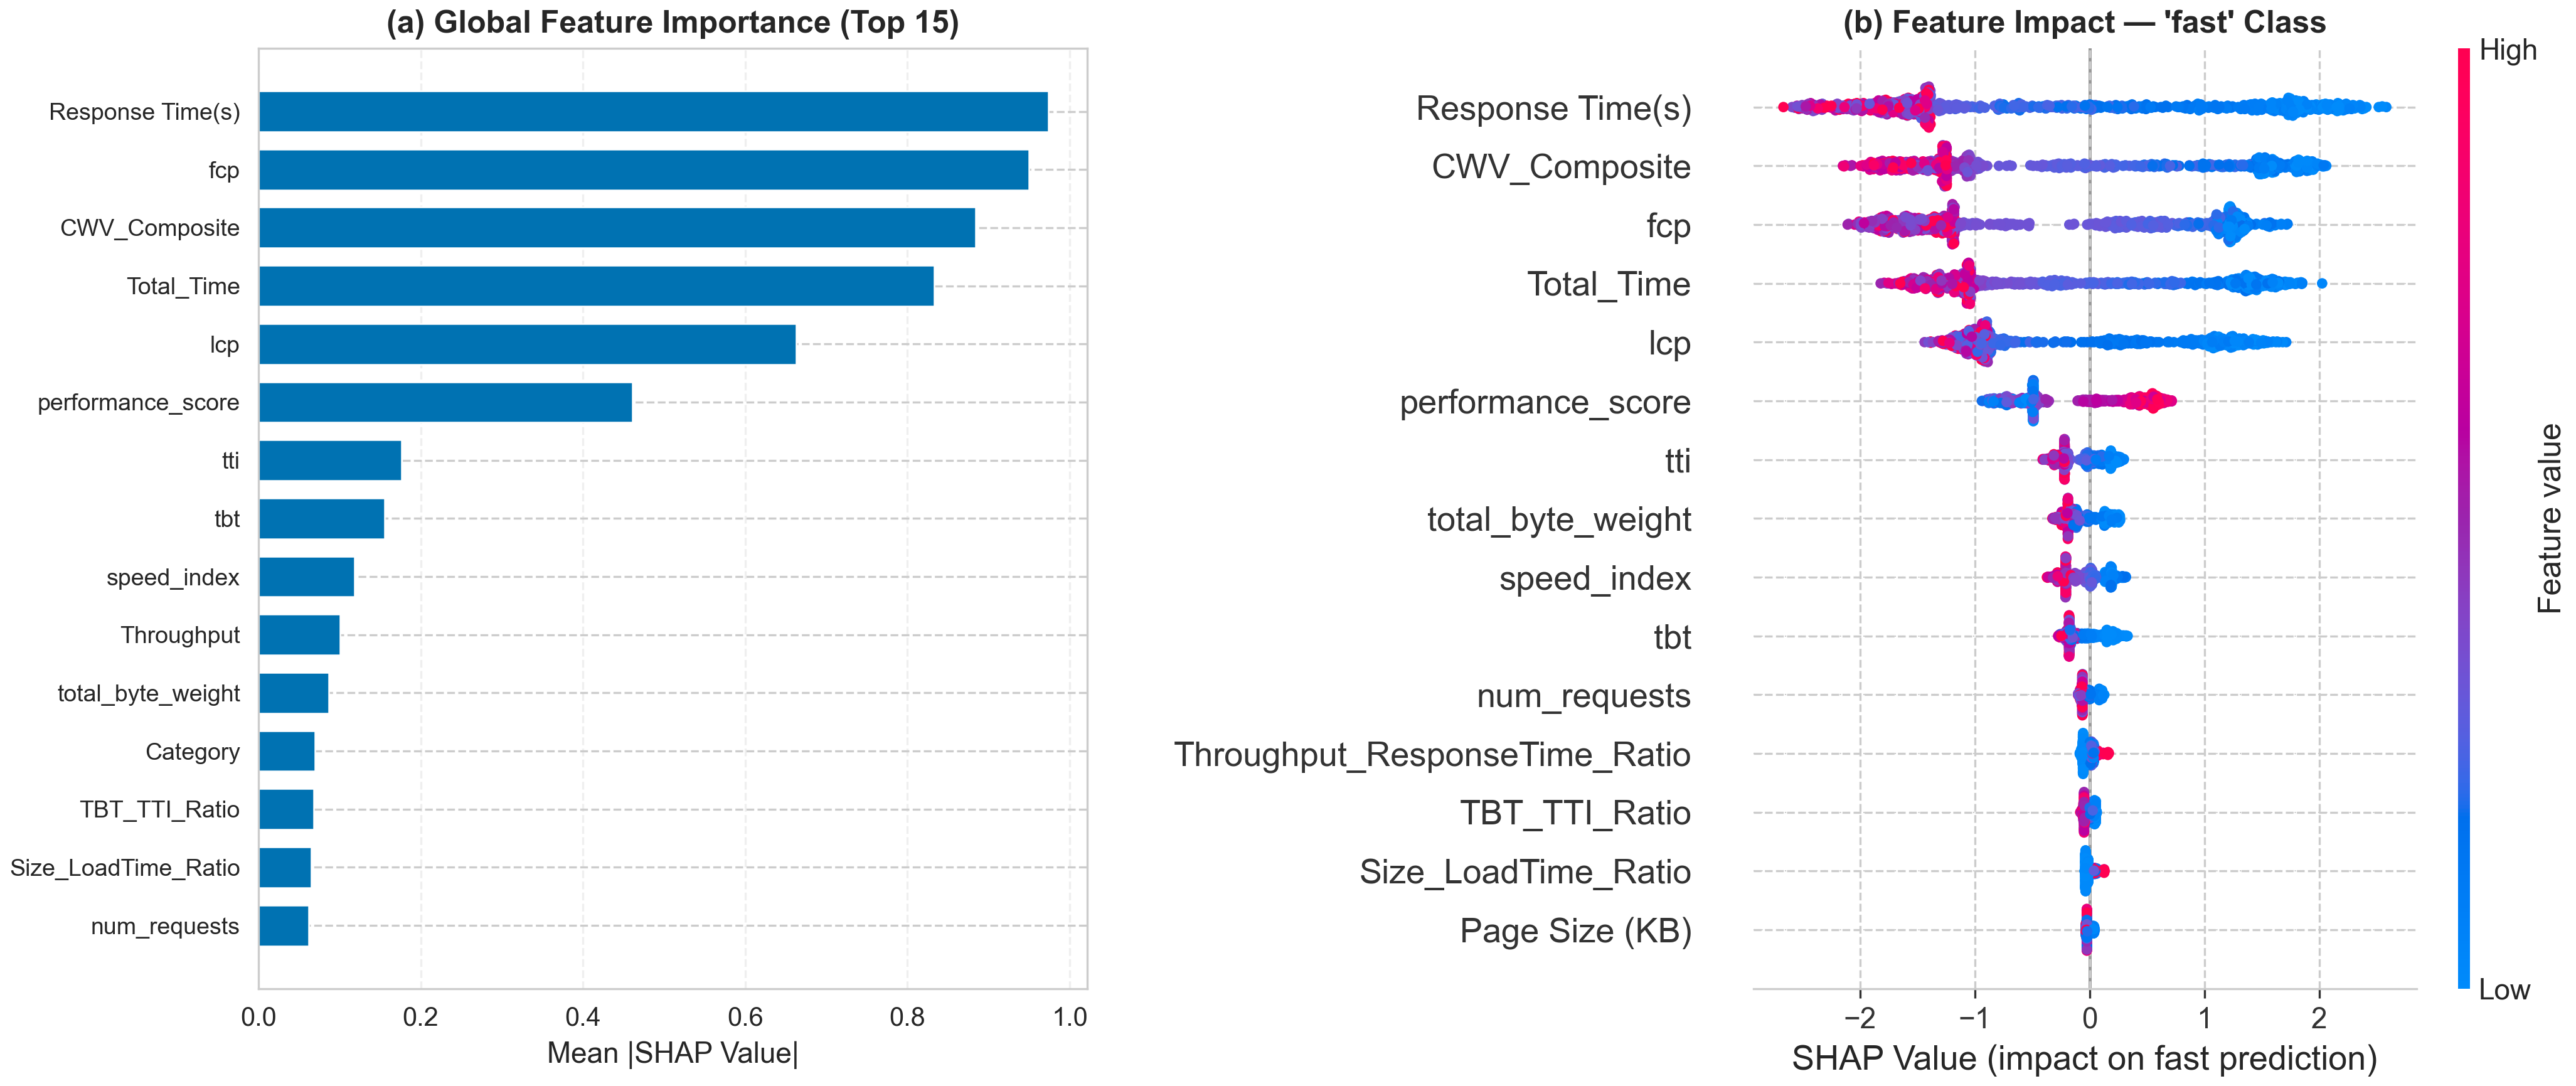
\includegraphics[width=\linewidth]{figures/fig2_shap_beeswarm.png}}
\caption{SHAP global feature importance showing the top 15 features ranked by mean absolute SHAP value. Core Web Vitals and latency indicators dominate, confirming the model learned domain-appropriate relationships.}
\label{fig:shap}
\end{figure}

We observed 100\% alignment on the top 5 features across methods. When the optimizer recommended reducing Total Byte Weight, LIME explicitly highlighted ``Page Size'' as the primary contributor to the Slow classification, providing a transparent reason code.

\subsection{Real-World Validation}
Table \ref{tab2} presents the results of the live deployment experiment. The AI-driven prescriptions translated into massive real-world gains, improving the Google PageSpeed score from 55 to 100.

\begin{table}[htbp]
\caption{Real-World Validation: Before vs. After Optimization}
\begin{center}
% The resizebox ensures the table fits exactly within the column width
\resizebox{\linewidth}{!}{%
\begin{tabular}{|c|c|c|c|}
\hline
\textbf{Metric}&\multicolumn{3}{|c|}{\textbf{Validation Results}} \\
\cline{2-4} 
\textbf{Name} & \textbf{\textit{Baseline (Slow)}}& \textbf{\textit{Optimized (Fast)}}& \textbf{\textit{Improvement}} \\
\hline
PageSpeed Score & 55/100 & 100/100 & +81.8\% \\
\hline
LCP (Loading) & 31.62 s & 0.85 s & -97.3\% \\
\hline
TBT (Interactivity) & 3 ms & 0 ms & -100.0\% \\
\hline
Page Size & 6.08 MB & 0.009 MB & -99.9\% \\
\hline
Model Conf. ($P_{fast}$) & 2.74\% & 99.74\% & +97.0 pp \\
\hline
\multicolumn{4}{l}{$^{\mathrm{a}}$Verified via external PageSpeed Insights API.}
\end{tabular}%
}
\label{tab2}
\end{center}
\end{table}

Figure~\ref{fig:pagespeed} shows the Google PageSpeed Insights screenshots confirming the external validation. The framework successfully reduced LCP by 97.3\%, validating that the prescriptive engine's theoretical adjustments result in tangible latency reductions in a production environment.

\begin{figure}[htbp]
\centering
\begin{minipage}[t]{0.48\linewidth}
    \centering
    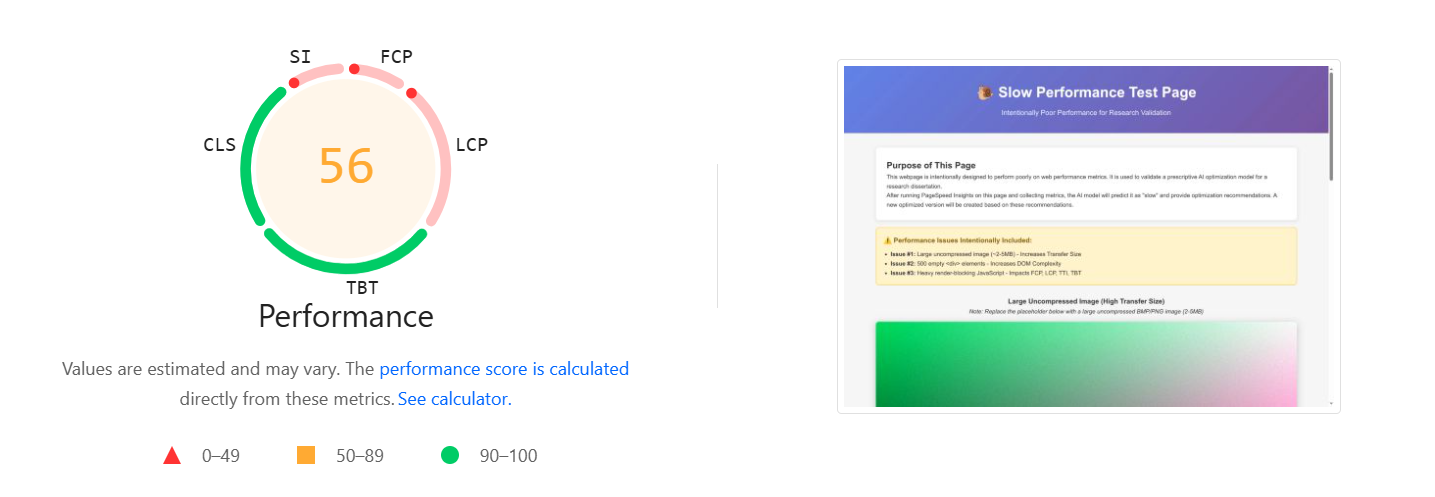
\includegraphics[width=\linewidth]{figures/slowpageperformance.png}
\end{minipage}
\hfill
\begin{minipage}[t]{0.48\linewidth}
    \centering
    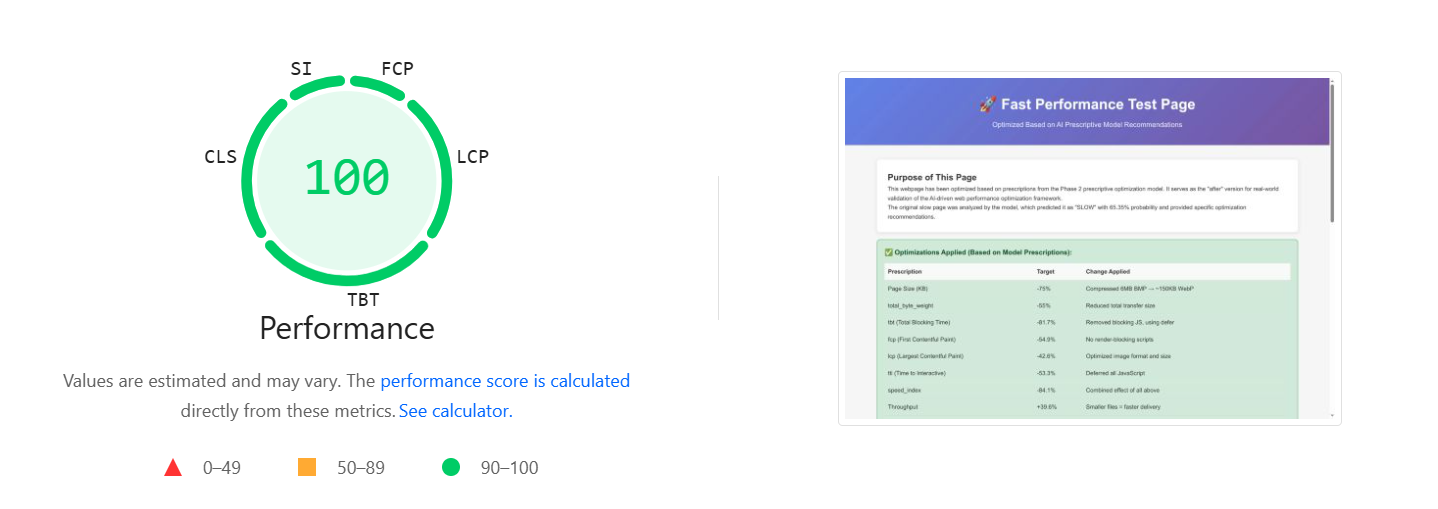
\includegraphics[width=\linewidth]{figures/fastpageperformance.png}
\end{minipage}
\caption{Google PageSpeed Insights: baseline (score 55, left) vs. optimised deployment (score 100, right). External audit independently verifies the framework's prescriptions with 94.5\% average metric improvement.}
\label{fig:pagespeed}
\end{figure}

\section{Discussion and Limitations}

This section interprets the experimental findings within the context of intelligent web engineering and addresses the constraints of the current study.

\subsection{Interpretation of Findings}
The integration of predictive modeling, prescriptive analytics, and XAI has yielded a framework that effectively bridges the gap between theoretical assessment and practical optimization.
\begin{itemize}
    \item \textbf{Validation of Prescriptive Power:} A critical contribution of this work is the empirical verification of optimization recommendations. While previous studies often stop at theoretical gain estimation, our real-world experiment demonstrated that the framework's advice is physically realizable. The observation that implementing the prescribed changes reduced the LCP by 97.3\% serves as definitive proof that the Differential Evolution engine identifies valid causal levers (e.g., asset compression) rather than spurious correlations.
    \item \textbf{Trust via Transparency:} The 100\% alignment between global (SHAP) and local (LIME) feature importance rankings suggests that the model’s reasoning is consistent. This transparency allows developers to audit the AI's thought process, ensuring that recommendations are made for the right reasons.
\end{itemize}

\subsection{Limitations}
Despite robust results, two key limitations define the scope of this work:
\begin{enumerate}
    \item \textbf{The ``Last Mile'' Problem:} The prescriptive engine identifies \textit{what} to change (e.g., ``Reduce JS payload by 200KB'') but not \textit{how} to refactor specific code. Recent LLM-based work \cite{burg2026} addresses this gap; our framework provides the quantified targets such systems require.
    \item \textbf{Dataset Scale:} Although enriched and externally validated on 8,000 URLs, edge cases in highly specific industries (e.g., WebGL-heavy gaming sites) may not be fully captured.
\end{enumerate}

\section{Conclusion and Future Work}

This research established a unified, empirically validated framework for web performance optimization. By integrating XGBoost classification, Differential Evolution, and Explainable AI, the proposed solution addresses the critical industry need for automated systems that not only detect bottlenecks but actively prescribe remedial actions.

\subsection{Summary of Contributions}
\begin{itemize}
    \item \textbf{Predictive-Prescriptive Integration:} We demonstrated an end-to-end pipeline where the classifier serves as a quality gate and fitness function for automated optimization, with explicit feature-to-action mapping.
    \item \textbf{External Validation:} Unlike prior simulation-based studies, we validated through cross-dataset transfer (97.54\% on 8,000 HTTP Archive URLs) and real-world deployment (PageSpeed \textbf{55$\rightarrow$100}).
    \item \textbf{Explainable Trust:} The fidelity-weighted consensus ranking reconciling SHAP, LIME, and Permutation Importance ensures stable, transparent reasoning.
\end{itemize}

\subsection{Future Directions}
Future work will focus on closing the loop between recommendation and implementation:
\begin{itemize}
    \item \textbf{LLM Integration:} Recent work on LLM-based DOM-level resolution \cite{burg2026} demonstrates that generative models can produce the code changes our framework specifies. Combining our quantified prescriptions with LLM code generation would close the ``last-mile'' gap from feature target to deployed fix.
    \item \textbf{Green Web Engineering:} Expanding the objective function to balance performance with energy efficiency.
    \item \textbf{Continuous Learning:} Online learning to adapt to evolving web standards in real-time.
\end{itemize}

% The references section follows immediately after this.

\section*{Acknowledgment}

The authors would like to express their sincere gratitude to COEP Technological University, Pune, for providing the academic environment and computational resources required to carry out this research.

\begin{thebibliography}{00}

% --- Predictive Modeling ---
\bibitem{ghattas2025}
M. Ghattas, A. M. Mora, and S. Odeh, ``A Novel Approach for Evaluating Web Page Performance Based on Machine Learning Algorithms and Optimization Algorithms,'' \textit{AI}, vol. 6, no. 2, p. 19, 2025.

\bibitem{sehwag2024}
A. Sehwag, A. P. Mishra, D. Kargeti, D. Pahadia, and G. Mangal, ``Applying Predictive Prefetching Using Deep Learning and NLP to Shorten Web Page Loading Times,'' \textit{Int. J. Multidiscip. Res. (IJFMR)}, vol. 6, no. 2, 2024.

\bibitem{mathur2024}
S. Mathur, Y. Hasan, D. Bhargava, S. Bhattacharjee, and A. Rana, ``Artificial Intelligence Based Predictive Analytics for Website Performance Optimization,'' in \textit{Proc. 7th Int. Conf. Contemp. Comput. Informat.}, 2024, pp. 795--800.

\bibitem{kaushik2024}
N. Kaushik, H. Kumar, and V. Raj, ``Micro Frontend Based Performance Improvement and Prediction for Microservices Using Machine Learning,'' \textit{J. Grid Comput.}, vol. 22, 2024.

\bibitem{xin2023}
R. Xin, H. Liu, P. Chen, and Z. Zhao, ``Robust and accurate performance anomaly detection and prediction for cloud applications: a novel ensemble learning-based framework,'' \textit{J. Cloud Comput.}, vol. 12, 2023.

\bibitem{dakic2025}
V. Daki\'{c}, G. Dambi\'{c}, J. Slovinac, and J. Red\v{z}epagi\'{c}, ``Optimizing Kubernetes Scheduling for Web Applications Using Machine Learning,'' \textit{Electronics}, vol. 14, no. 5, p. 863, 2025.

\bibitem{huang2023}
D. Huang, L. Costero, A. Pahlevan, M. Zapater, and D. Alonso, ``Cloud Prophet: A Machine Learning-Based Performance Prediction for Public Clouds,'' \textit{IEEE Trans. Sustain. Comput.}, 2023.

\bibitem{vanriet2023}
J. van Riet, I. Malavolta, and T. A. Ghaleb, ``Optimize along the way: An industrial case study on web performance,'' \textit{J. Syst. Softw.}, vol. 198, p. 111593, 2023.

% --- Prescriptive Optimization ---
\bibitem{notz2024}
P. M. Notz and R. Pibernik, ``Explainable subgradient tree boosting for prescriptive analytics in operations management,'' \textit{Eur. J. Oper. Res.}, vol. 312, no. 3, pp. 1119--1133, 2024.

\bibitem{surianarayanan2023}
C. Surianarayanan, J. J. Lawrence, P. R. Chelliah, E. Prakash, and C. Hewage, ``A Survey on Optimization Techniques for Edge Artificial Intelligence (AI),'' \textit{Sensors}, vol. 23, no. 3, p. 1279, 2023.

\bibitem{goscien2025}
R. Go\'{s}cie\'{n}, ``Explainable artificial intelligence-based framework for efficient content placement in elastic optical networks,'' \textit{Expert Syst. Appl.}, vol. 262, p. 125541, 2025.

\bibitem{asha2025}
M. M. Asha and G. Ramya, ``Predator crow search optimization with explainable AI for cardiac vascular disease classification,'' \textit{Sci. Rep.}, vol. 15, 2025.

\bibitem{liu2023}
B. Liu et al., ``AI-DeMat: A web-based expert system platform for computationally expensive models in materials design,'' \textit{Adv. Eng. Softw.}, vol. 176, p. 103361, 2023.

% --- Explainable AI (XAI) ---
\bibitem{salih2024}
A. M. Salih et al., ``A Perspective on Explainable Artificial Intelligence Methods: SHAP and LIME,'' 2024, \textit{Preprint}, arXiv:2305.02012.

\bibitem{goldwasser2024}
J. Goldwasser and G. Hooker, ``Provably Stable Feature Rankings with SHAP and LIME,'' 2024, \textit{Preprint}, arXiv:2401.15800.

\bibitem{hassija2024}
V. Hassija et al., ``Interpreting Black-Box Models: A Review on Explainable Artificial Intelligence,'' \textit{Cogn. Comput.}, vol. 16, pp. 45--74, 2024.

\bibitem{mersha2024}
M. Mersha, K. N. Lam, J. Wood, A. AlShami, and J. Kalita, ``Explainable artificial intelligence: A survey of needs, techniques, applications, and future direction,'' \textit{Neurocomputing}, vol. 599, 2024.

\bibitem{bennetot2024}
A. Bennetot et al., ``A Practical Tutorial on Explainable AI Techniques,'' \textit{ACM Comput. Surv.}, vol. 57, 2024.

\bibitem{ortigossa2024}
E. Ortigossa, T. Gonçalves, and L. Nonato, ``EXplainable Artificial Intelligence (XAI) - From Theory to Methods and Applications,'' \textit{IEEE Access}, vol. 12, pp. 80799--80846, 2024.

\bibitem{ali2023}
S. Ali et al., ``Explainable Artificial Intelligence (XAI): What we know and what is left to attain Trustworthy Artificial Intelligence,'' \textit{Inf. Fusion}, vol. 99, p. 101805, 2023.

\bibitem{mersha2025}
M. Mersha et al., ``Explainable AI: XAI-guided context-aware data augmentation,'' \textit{Expert Syst. Appl.}, vol. 289, p. 128364, 2025.

\bibitem{alam2024}
K. Alam et al., ``SXAD: Shapely eXplainable AI-Based Anomaly Detection Using Log Data,'' \textit{IEEE Access}, vol. 12, pp. 95659--95672, 2024.

\bibitem{benleulmi2025}
M. Benleulmi, I. Gasmi, N. Azizi, and N. Dey, ``Explainable AI and Deep Learning Models for Recommender Systems: State of the Art and Challenges,'' \textit{J. Univers. Comput. Sci.}, vol. 31, no. 4, pp. 383--421, 2025.

\bibitem{goyal2025}
B. Goyal, ``Explainable AI (XAI) for Cloud-Based Enterprise Applications: Building Trust and Transparency in AI-Driven Decisions,'' \textit{J. Int. Crisis Risk Commun. Res.}, vol. 8, no. S9, pp. 63--71, 2025.

% --- LLM-Based Approaches ---
\bibitem{burg2026}
L. Burg, Q. Ye, and A. Hindle, ``Evaluating the Use of LLMs for Automated DOM-Level Resolution of Web Performance Issues,'' in \textit{Proc. 23rd IEEE/ACM Int. Conf. Mining Softw. Repositories (MSR)}, 2026.

\end{thebibliography}

\end{document}
